\documentclass[tikz,border=10pt]{standalone}
\usepackage{amsmath}
\usetikzlibrary{automata,positioning,arrows.meta,calc}
\begin{document}
\begin{minipage}{15cm}
\centering
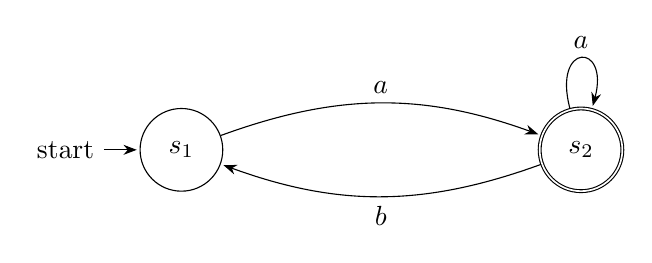
\begin{tikzpicture}[
  >=Stealth,
  shorten >=1pt,
  node distance=4cm,
  auto,
  every state/.style={minimum size=1.05cm}
]
  \node[state,initial] (s1) {$s_1$};
  \node[state,accepting,right=of s1] (s2) {$s_2$};

  \path[->]
    (s1) edge[bend left=20] node {$a$} (s2)
    (s2) edge[bend left=20] node {$b$} (s1)
         edge[loop above] node {$a$} ();

\end{tikzpicture}
\par\vspace{1.5em}
$\displaystyle
  M(a)=\begin{pmatrix}0&1\\0&1\end{pmatrix}
  \qquad
  M(b)=\begin{pmatrix}0&0\\1&0\end{pmatrix}
  \qquad
  v_I=\begin{pmatrix}1&0\end{pmatrix}
  \qquad
  v_F=\begin{pmatrix}0\\1\end{pmatrix}
$
\end{minipage}
\end{document}
